% All the result and analysis
\chapter{The Results}
\label{chapter:results}
\begin{quote}
\textsl{``The most incomprehensible thing about the world is that it is comprehensible." - Albert Einstein}
\end{quote}

\section{Introduction}
It is always a challenge to extract and analyze data from an Artificial Life simulation. Data and analysis in this simulation has been concentrated on evaluating whether evolution of mimicry has taken place. This evaluation can be made with the number of different rings that has been created and the size of each of those rings along with the population of palatable and unpalatable species. Also it can be established whether Batesian Mimicry and Mullerian Mimicry has taken effect by analyzing the data set of these populations.

\section{Mimicry Ring Reports}
The mimicry ring reports consist entirely of the population of prey species categorized according to pattern and palatability. Data is stored at every instance of time of the simulation keeping an interval of 10 iterations. As the number of rings that get generated reaches as many as 50 or more, and all the population of ring do not last for the entire simulation, so while storing data we have taken the most populous of the surviving 8 rings to plot. Parameters are mentioned in table \ref{tab:ring-report-control-parameters}.

\begin{table}[H]
\centering
\begin{tabular}{| p{2cm} | >{\centering} p{2.2cm} | p{8cm} |}
	\hline
		\textbf{Parameter} & \textbf{Value} & \textbf{Description} \\ \hline
		Mimicry Ring Hamming Distance & 10 \% of the Pattern Size & If the Hamming distance between the pattern of the model and the mimic is 10 \% the size of the pattern then they are considered within the same ring.\\ \hline
		Number of Rings to report & 8 & This value is the number of most populous rings that are included in the report.\\
	\hline
\end{tabular}
\caption{Parameters to mimicry ring report.}
\label{tab:ring-report-control-parameters}
\end{table}

\section{Initial configuration with two prey species}
\label{sec:init-conf-2prey}
% Put the table here
\begin{table}[H]
\centering
\begin{tabular}{|l|l|c|c|l|c|}
  \hline
   														&\multicolumn{3}{|c|}{Prey configuration} 																	
   														& \multicolumn{2}{|c|}{Predator configuration} \\ \hline
  \multirow{2}{*}{Population} & Rule110 (Palatable) & \parbox[c]{2.1em}{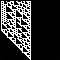
\includegraphics[scale=0.50]{images/CARule110}} & 108 
  														& \multicolumn{2}{|c|}{\multirow{2}{*}{10}} \\ \cline{2-4}
  					 									& Rule30 (Unpalatable)& \parbox[c]{2.1em}{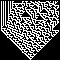
\includegraphics[scale=0.50]{images/CARule30}}  & 108 
  					 									& \multicolumn{2}{|c|}{}\\ \hline
  \multirow{2}{*}{Reproduction} & Age Limit & \multicolumn{2}{|c|}{100}  & \multicolumn{2}{|c|}{500} \\ \cline{2-6}
  						 									& Interval  & \multicolumn{2}{|c|}{1000} & \multicolumn{2}{|c|}{1200} \\ \hline
  \multirow{2}{*}{Mutation Rate} & Pattern   & \multicolumn{2}{|c|}{0.05} & \multicolumn{2}{|c|}{\multirow{2}{*}{0.3}} \\ \cline{2-4}
  						 									 & Genome    & \multicolumn{2}{|c|}{0.5}  & \multicolumn{2}{|c|}{} \\ \hline
  Demise Age	 									 & \multicolumn{3}{|c|}{2000}							& \multicolumn{2}{|c|}{2500} \\ \hline
  Minimum Attack Age						 & \multicolumn{3}{|c|}{} 						    & \multicolumn{2}{|c|}{500} \\ \hline
  \multirow{2}{*}{Memory Configuration} & \multicolumn{3}{|c|}{} 					& Minimum & 2 \\ \cline{5-6}
   																			& \multicolumn{3}{|c|}{} 					& Maximum & 10 \\ \hline  
\end{tabular}
\caption{Agent configuration of 2 prey species}
\label{tab:config-table-2-prey}
\end{table}

The set of parameters in table \ref{tab:config-table-2-prey} were carefully selected to be the initial condition for this run of the simulation. This test has been done with two sets of prey species with very different CA pattern and with opposite palatability and equal population. To control reproduction of the prey species their age limit has been set to 100 iterations into the time the species were alive. And the reproduction interval was set to 1000 iterations.

Pattern mutation rate has been set to a minimal level of 0.05 as by increasing this variable it is possible to increase the size of the number of mimicry rings present in the simulation. The genome mutation rate controls the rate at which genome of the child prey species will deviate from their parents. As mentioned earlier the genome mutation rate has been separated from the pattern mutation rate to bring more control to the number of mimicry rings generated.

Prey demise age has been kept to 2000 iterations while predator demise age is set to 2500. But in the later experiments predator demise age has been increased to 5000 iterations. Predators in this simulation generate selection pressure for the evolution of mimicry. So the longer a predator is present in the simulation it will be making intelligent decisions in term of selecting which prey species to consume and which one to avoid. But with the current rate of demise for predator we were able to create successful mimetic population of prey species as we will see in the analysis in the following results.

Initial population of predator species has been set to 10 which is in accordance with the prey population in the simulation. The reason for such low number of predator is, unlike prey species which are consumed by predators, there is no cause for the predator species to die accept their natural cause of death, that is to reach their demise age. So predator population can explode very easily. That is why their population is controlled in a restrictive manner with the help of high reproduction age limit and reproduction age interval.

The memory configuration size for predators is a very interesting parameter. The minimum memory size is directly associated with the number of prey species with which we initiate the simulation. Otherwise evolution of mimicry is not observed. As mentioned in table \ref{tab:predator-control-parameters} the minimum memory size is the number of prey species predator would consume before starting to make decisive consumption of prey species. After the initial birth of a predator and when the minimum attack age is crossed, it starts consuming prey species present in its vicinity without making any judgment. At this point its memory size is zero. As long as the minimum memory size is not reached predators will blindly consume prey species and insert their CA pattern and associated palatability into its Hopfield memory bank. No later than the minimum memory size has been reached, predators will start making intelligent decision about consuming its prey species. When catching a prey if its memory tells that it is palatable, it will consume that prey. Otherwise if memory recognizes it to be unpalatable predator will certainly let it go.

Now as we know the behavior of Hopfield memory, a recognition result will always be achieved depending on the similarity of the patterns stored in memory. So when minimum memory size has been reached the predator will always make a decision based on the similarity of the prey pattern currently captured and the patterns stored in memory.

% Put the image
\begin{figure}[H]
	\centering
	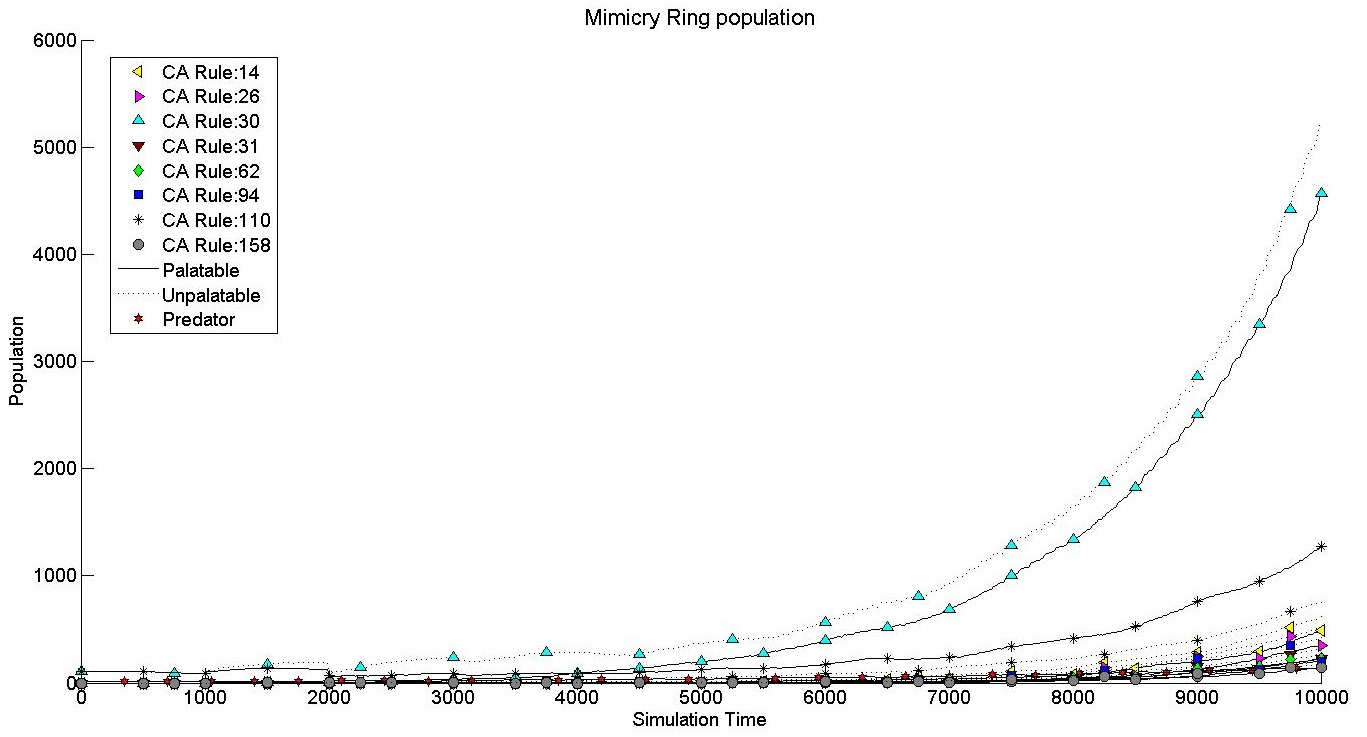
\includegraphics[scale=0.40]{images/simTime10k-2Prey}
	\caption[Population distribution of mimicry rings (2 prey species, 10k iterations)]{Population distribution of mimicry rings, initialized with 2 prey species, 10k iterations}
	\label{fig:plot-2-prey}
\end{figure}

The plot in Figure \ref{fig:plot-2-prey} is simulation time verses prey population after running it for 10000 iterations. With the initial configuration in the above table we can observe that multiple rings of prey population have been created. Two prey species are considered to be in a ring if their CA pattern have a hamming distance within 10 bits. This parameter is mentioned in table \ref{tab:ring-report-control-parameters}. Population of palatable species has been represented with line curve while population of unpalatable species has been presented with dotted curve. Different signs of squares, triangles and diamonds have been used to distinguish between species of prey population. The simulation was initiated with two prey species having CA rule of 30 and 110 and being palatable and unpalatable consecutively.

\begin{figure}[H]
	\centering
	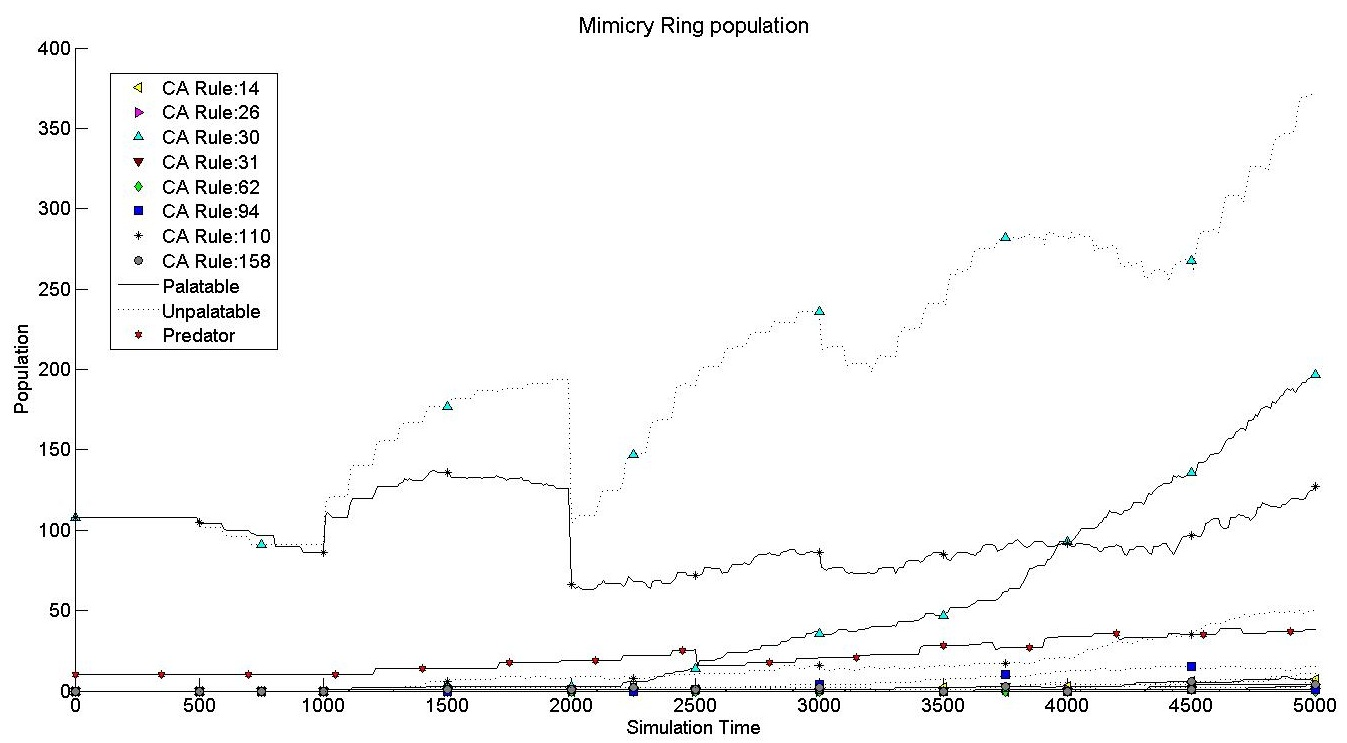
\includegraphics[scale=0.40]{images/simTime5k-2Prey}
	\caption[Population distribution of mimicry rings (2 prey species, 5k iterations)]{Population distribution of mimicry rings, initialized with 2 prey species, 5k iterations.}
	\label{fig:plot-2-prey-5k}
\end{figure}

The plot of figure \ref{fig:plot-2-prey-5k} is from the same experiment as of figure \ref{fig:plot-2-prey}, but only up to 5000 iterations. By closely observing the graph of figure \ref{fig:plot-2-prey-5k}, we could see the population of two species have started dropping at around time 500 when the initial predator population reaches the maturity for consuming prey species (effect of the parameter `Minimum Attack Age' from table \ref{tab:config-table-2-prey}). At around time 1000 the prey population starts reproducing as the population increases (controlled by `Reproduction Age Limit' from table \ref{tab:config-table-2-prey}). At the same time different other species of prey gets to be born with mutated CA patterns. There is a straight drop of prey population at time 2000, when all the prey species with which the simulation was initialized come to its demise age (controlled by `Prey Demise Age' at table \ref{tab:config-table-2-prey}). Over time the population of CA Rule 30 dominates the population (figure \ref{fig:plot-2-prey}) as most predators recognize it as unpalatable. Similarly a palatable population of CA Rule 30 or within the same ring of palatable species starts rising, while at one point overlaps the population of CA Rule 110 (Time: 4000 approx.). CA Rule 110 was initialized as a set of palatable species.

We can observe from the above result that the evolution of mimicry has taken effect. A population of mimics were successfully able to exceed the population of other prey species, and the reason being, avoidance by predators of prey pattern similar to unpalatable ones. We can conclude that Batesian mimicry has taken effect in the simulation.

%Put the number of rings picture:
\begin{figure}[H]
	\centering
	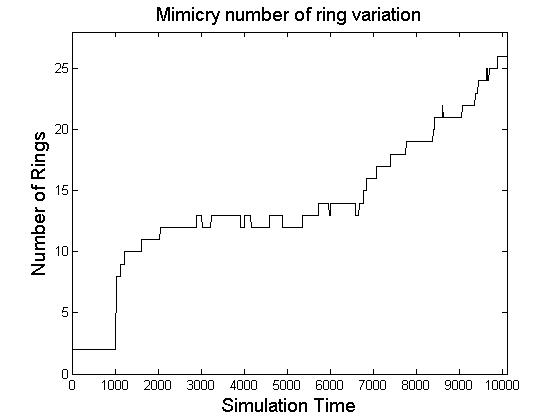
\includegraphics[scale=0.50]{images/ringSize10k-2Prey}
	\caption[Number of mimicry rings (2 prey species)]{Number of mimicry rings, initialized with 2 prey species.}
	\label{fig:ringSize10k-2Prey}
\end{figure}

Observing from figure \ref{fig:ringSize10k-2Prey} the number of rings in this simulation makes a slow increase from 2 at the initial configuration to 27 rings at the end of 10000 iterations. A small change in CA genetic representation can have a very large effect in terms of the phenotype of the pattern with which the prey is represented. For example if we take a look at the set of pattern genotype with very different phenotype in table \ref{tab:diff-in-pattern}.

%CARule table
\begin{table}[H]
\centering
\begin{tabular}{|l|c|c|c|}
  \hline
  CA Rule & \(60 \equiv 00111100\) & \(61 \equiv 00111101\) & \(62 \equiv 00111110 \) \\ \hline
  Pattern & \parbox[c]{2.1em}{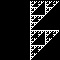
\includegraphics[scale=0.50]{images/CARule60}} 
  				& \parbox[c]{2.1em}{
\includegraphics[scale=0.50]{images/CARule61}} 
  				& \parbox[c]{2.1em}{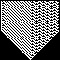
\includegraphics[scale=0.50]{images/CARule62}}\\
  \hline
\end{tabular}
\caption{Difference in prey pattern genotype and phenotype}
\label{tab:diff-in-pattern}
\end{table}

All the patterns in table \ref{tab:diff-in-pattern} have a genetic bit difference of 1. So by a single mutation there can be three different set of phenotype for a child organism from its parent. This is largely the reason for the increased number of mimicry rings created in the simulation. Only the 8 most populous rings are presented in the graphs with population verses simulation time.

\begin{figure}[H]
	\centering
	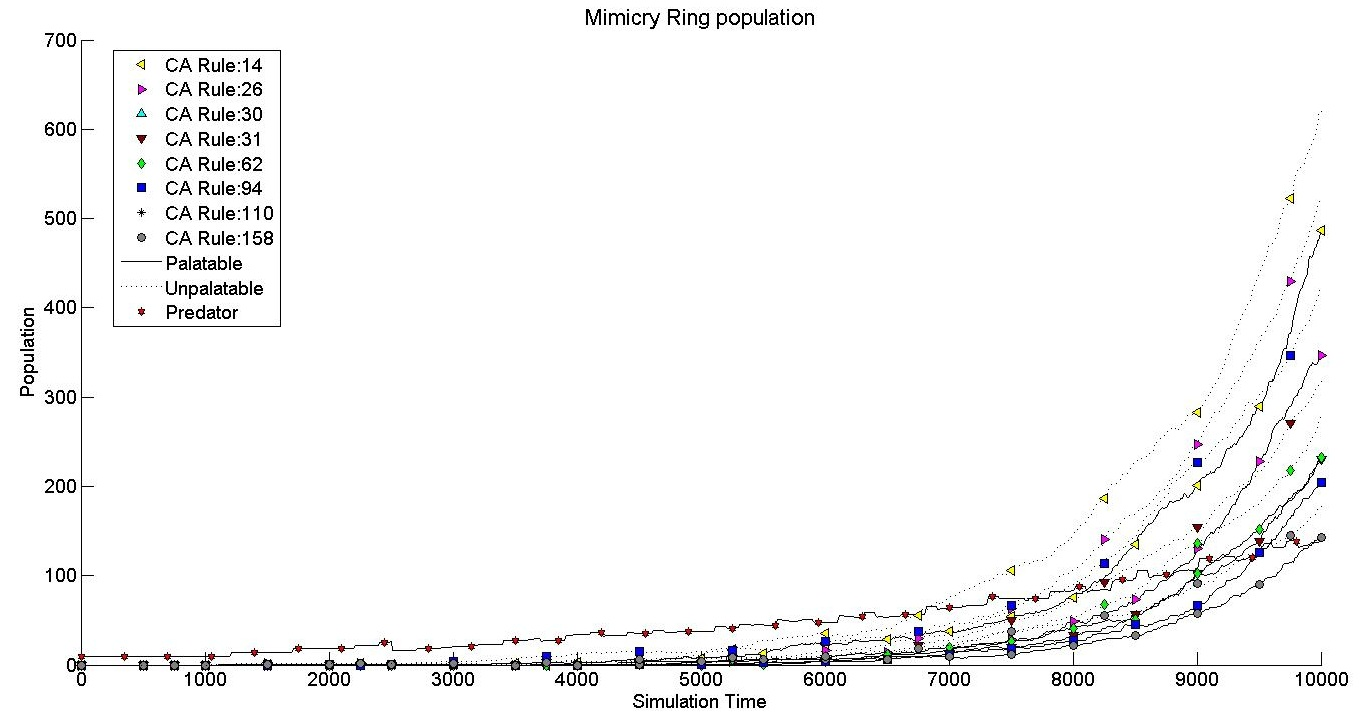
\includegraphics[scale=0.40]{images/simTime10k-2Prey-generated-prey}
	\caption[Population distribution of generated mimicry rings (2 prey species)]{Population distribution of generated mimicry rings, initialized with 2 prey species.}
	\label{fig:plot-2-prey-generated-prey}
\end{figure}

Figure \ref{fig:plot-2-prey-generated-prey} is the same experimental data of figure \ref{fig:plot-2-prey} but with only the newly generated ring of prey species. The initialized dominant population of CA rule 110 and 30, both palatable and unpalatable has been eliminated from this graph to observe the newly created rings. In this plot, among the population of new patterns the unpalatable ones dominate (CA Rule 14, 26, 94). Also the palatable counterpart of the unpalatable population is increasing their number. Species with \textsl{un-mimicked} palatable pattern is very few in number.

The screen shot in figure \ref{fig:screenshot-simTime7600-2-prey} is for one instance of time of the simulation. The red agents are predators while the black agents with different textured patterns are the prey species. According to their behavior most of the prey species are flocking together in a group while also being chased by the predators, whose sole purpose is to consume prey species. 

%Screenshot of the simulation
\begin{figure}[H]
	\centering
	\label{fig:screenshot-simTime7600-2-prey}
	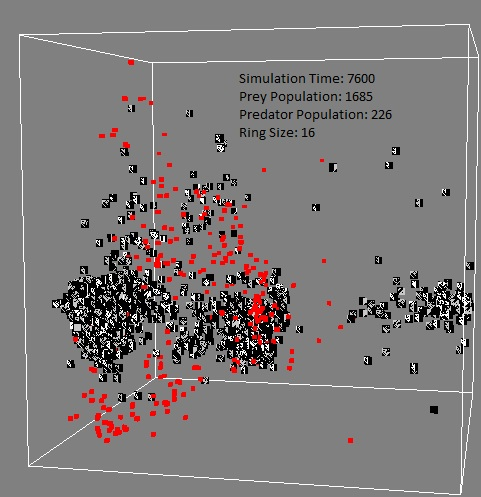
\includegraphics[scale=0.55]{images/simTime7600}
	\caption[Graphical representation of the model (simulation time: 7600)]{Graphical representation of the model, simulation time: 7600.}
\end{figure}

\section{Initial configuration with four prey species}
\begin{table}[H]
\centering
\begin{tabular}{|l|l|c|c|l|c|}
  \hline
   														&\multicolumn{3}{|c|}{Prey configuration} 																	
   														& \multicolumn{2}{|c|}{Predator configuration} \\ \hline
  \multirow{4}{*}{Population} & Rule110 (Unpalatable) & \parbox[c]{2.1em}{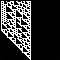
\includegraphics[scale=0.50]{images/CARule110}} 
  																										& 50 & \multicolumn{2}{|c|}{\multirow{4}{*}{10}} \\ \cline{2-4}
  					 									& Rule30 (Palatable)& \parbox[c]{2.1em}{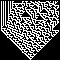
\includegraphics[scale=0.50]{images/CARule30}}
  					 																					& 50 & \multicolumn{2}{|c|}{}\\ \cline{2-4}
  					 									& Rule55 (Unpalatable)& \parbox[c]{2.1em}{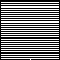
\includegraphics[scale=0.50]{images/CARule55}}
  					 																					& 50 & \multicolumn{2}{|c|}{}\\ \cline{2-4}
  					 									& Rule190 (Palatable)& \parbox[c]{2.1em}{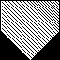
\includegraphics[scale=0.50]{images/CARule190}}
  					 																					& 50 & \multicolumn{2}{|c|}{}\\ \hline
  \multirow{2}{*}{Reproduction} & Age Limit & \multicolumn{2}{|c|}{100}  & \multicolumn{2}{|c|}{500} \\ \cline{2-6}
  						 									& Interval  & \multicolumn{2}{|c|}{1000} & \multicolumn{2}{|c|}{1400} \\ \hline
  \multirow{2}{*}{Mutation Rate} & Pattern   & \multicolumn{2}{|c|}{0.05} & \multicolumn{2}{|c|}{\multirow{2}{*}{0.3}} \\ \cline{2-4}
  						 									 & Genome    & \multicolumn{2}{|c|}{0.5}  & \multicolumn{2}{|c|}{} \\ \hline
  Demise Age	 									 & \multicolumn{3}{|c|}{2000}							& \multicolumn{2}{|c|}{2500} \\ \hline
  Minimum Attack Age						 & \multicolumn{3}{|c|}{} 						    & \multicolumn{2}{|c|}{500} \\ \hline
  \multirow{2}{*}{Memory Configuration} & \multicolumn{3}{|c|}{} 					& Minimum & 4 \\ \cline{5-6}
   																			& \multicolumn{3}{|c|}{} 					& Maximum & 10 \\ \hline  
\end{tabular}
\caption{Agent configuration of 4 prey species}
\label{tab:config-table-4-prey}
\end{table}

This run of the simulation has been initialized with four prey species with very different CA pattern configuration. The predator reproduction interval has been increased to 1400, while the minimum memory size has been increased to 4 instead of 2 as the predator is expected to memorize four different species of prey before starting to make intelligent decision about consuming them. The rest of the parameters remain the same as from the experiment in section \ref{sec:init-conf-2prey}.

\begin{figure}[H]
	\centering
	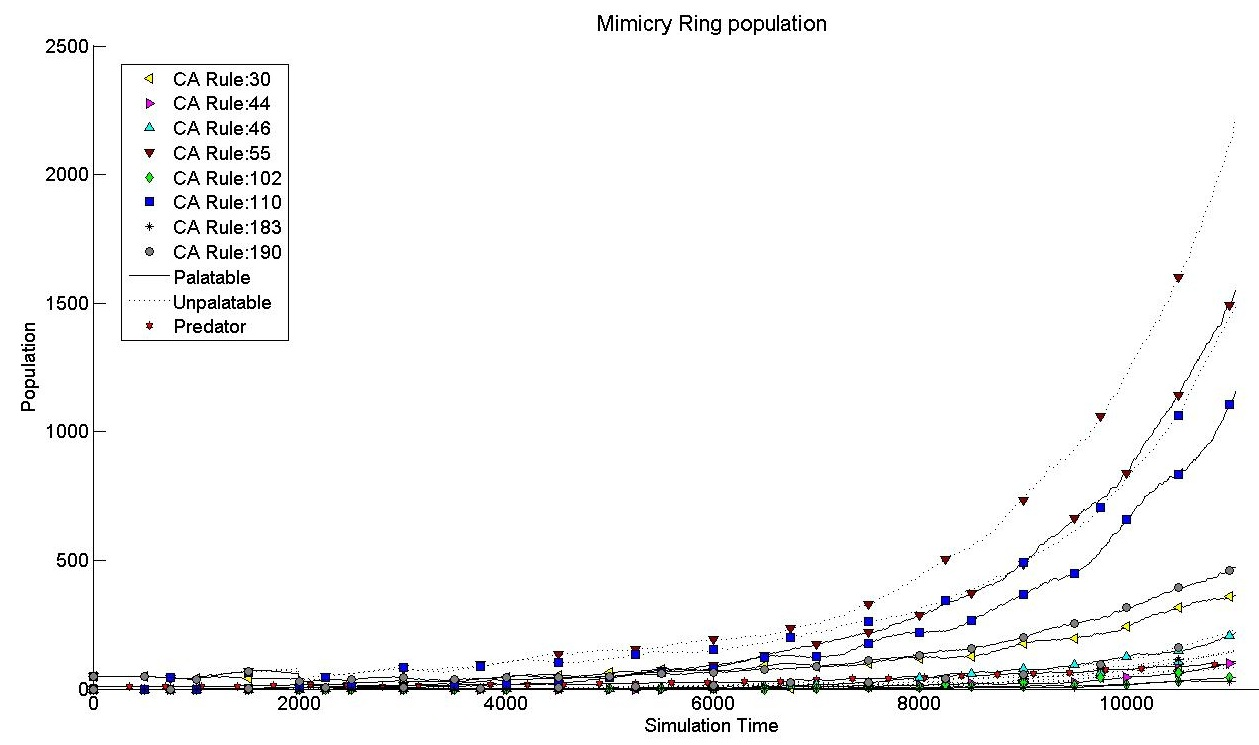
\includegraphics[scale=0.40]{images/simTime10k-4Prey}
	\caption[Population distribution of mimicry rings (4 prey species)]{Population distribution of mimicry rings, initialized with 4 prey species.}
	\label{fig:plot-4-prey}
\end{figure}

By observing the graph in figure \ref{fig:plot-4-prey} we can see the two rings of unpalatable species (CA Rule 55, 110) which was put at the initial sate of the simulation has dominated after 10000 iterations. CA rule 55 has taken over all other species while CA 110 is following it (represented with dotted curve). Also the palatable prey species with similar patterns to CA rule 55 and 110 are taking full advantage of their deceiving pattern and increasing their population (represented with line curve). The two palatable set of patterns CA Rule 190 and 30 are unable to dominate the population. Different other mimicry rings are present in the simulation as we can observe from the graph of number of rings verses simulation time in figure \ref{fig:ringSize10k-4Prey}. The total number of rings reached somewhere near 37 while most of them have comparatively low representative population. Batesian mimicry is in full effect in this simulated environment.

\begin{figure}[H]
	\centering
	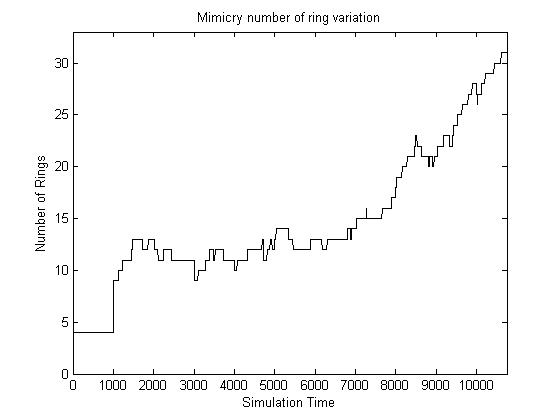
\includegraphics[scale=0.50]{images/ringSize10k-4Prey}
	\caption[Number of mimicry rings (4 prey species)]{Number of mimicry rings, initialized with 4 prey species.}
	\label{fig:ringSize10k-4Prey}
\end{figure}

\begin{figure}[H]
	\centering
	\label{fig:screenshot-simTime11K-4Prey}
	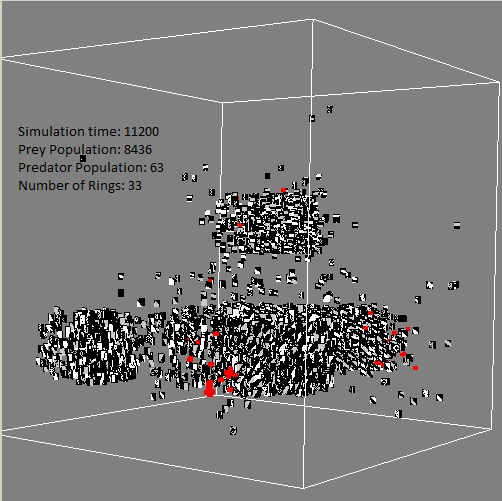
\includegraphics[scale=0.55]{images/simTime11K-4Prey}
	\caption[Graphical representation of the model (simulation time: 11200)]{Graphical representation of the model initialized with 4 prey species, simulation time: 11200.}
\end{figure}

\section{Increased initial population with four prey species}

\begin{table}[H]
\centering
\begin{tabular}{|l|l|c|c|l|c|}
  \hline
   														&\multicolumn{3}{|c|}{Prey configuration} 																	
   														& \multicolumn{2}{|c|}{Predator configuration} \\ \hline
  \multirow{4}{*}{Population} & Rule110 (Palatable) & \parbox[c]{2.1em}{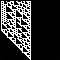
\includegraphics[scale=0.50]{images/CARule110}} & 150 & \multicolumn{2}{|c|}{\multirow{4}{*}{20}} \\ \cline{2-4}
  					 									& Rule30 (Palatable)& \parbox[c]{2.1em}{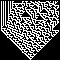
\includegraphics[scale=0.50]{images/CARule30}}  	 & 150 & \multicolumn{2}{|c|}{}\\ \cline{2-4}
  					 									& Rule55 (Unpalatable)& \parbox[c]{2.1em}{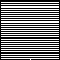
\includegraphics[scale=0.50]{images/CARule55}}  & 150 & \multicolumn{2}{|c|}{}\\ \cline{2-4}
  					 									& Rule190 (Unpalatable)& \parbox[c]{2.1em}{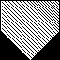
\includegraphics[scale=0.50]{images/CARule190}}& 150 & \multicolumn{2}{|c|}{}\\ \hline
  \multirow{2}{*}{Reproduction} & Age Limit & \multicolumn{2}{|c|}{100}  & \multicolumn{2}{|c|}{500} \\ \cline{2-6}
  						 									& Interval  & \multicolumn{2}{|c|}{1000} & \multicolumn{2}{|c|}{2500} \\ \hline
  \multirow{2}{*}{Mutation Rate} & Pattern   & \multicolumn{2}{|c|}{0.05} & \multicolumn{2}{|c|}{\multirow{2}{*}{0.3}} \\ \cline{2-4}
  						 									 & Genome    & \multicolumn{2}{|c|}{0.5}  & \multicolumn{2}{|c|}{} \\ \hline
  Demise Age	 									 & \multicolumn{3}{|c|}{2000}							& \multicolumn{2}{|c|}{7000} \\ \hline
  Minimum Attack Age						 & \multicolumn{3}{|c|}{} 						    & \multicolumn{2}{|c|}{500} \\ \hline
  \multirow{2}{*}{Memory Configuration} & \multicolumn{3}{|c|}{} 					& Minimum & 4 \\ \cline{5-6}
   																			& \multicolumn{3}{|c|}{} 					& Maximum & 10 \\ \hline  
\end{tabular}
\caption{Agent configuration of 4 prey species with increased population}
\label{tab:config-table-4-more-prey}
\end{table}

In this run of the simulation some significant parameters have been updated. First one is the initial population of prey species. It has been increased from 50 to 150 for each of the prey species, while increasing the overall population from 200 to 600. Secondly the number of predator population has been increased from 20 to 30. Thirdly, predator demise age has been increased from 2500 to 7000 while their reproduction interval has been increased from 1400 to 2500. Increasing predator demise age can have an interesting effect, as the longer a predator is present in a simulation, the longer it will be making intelligent decision in terms of consuming its prey and there will be increased selection pressure from the entire population of predators. 

\begin{figure}[H]
	\centering
	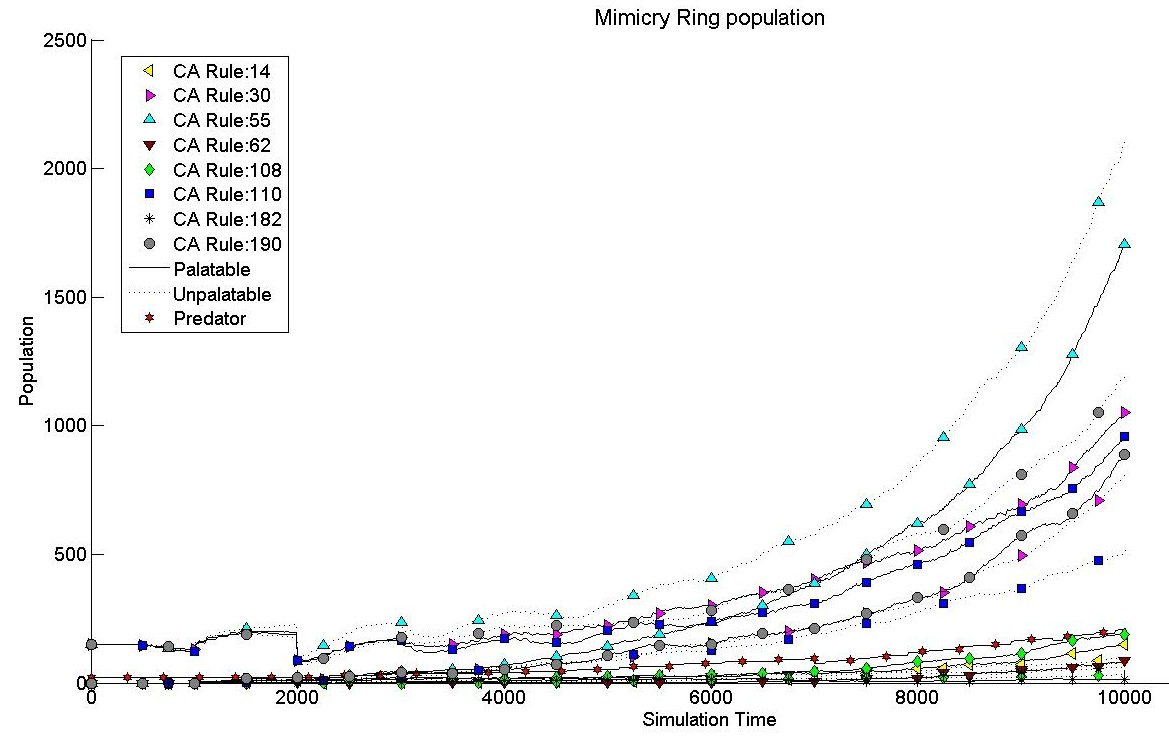
\includegraphics[scale=0.45]{images/simTime10K-4MorePrey}
	\caption[Population distribution of mimicry rings (4 prey species, increased population)]{Population distribution of mimicry rings, initialized with 4 prey species with increased population.}
	\label{fig:plot-4-more-prey}
\end{figure}

Some very interesting diversity of mimicry rings can be observed in the simulation for updating these parameters. The unpalatable rings and their deceptive counterparts (palatable prey with similar pattern) still have their dominance. We can observe CA Rule 55 and 190 are the highest in number of population. Interestingly enough CA Rule 30 and 110 which started as palatable prey species has also taken dominance in the simulation, following 55 and 190. The unpalatable counter part of CA Rule 30 and 110 are also following the palatable population. 

The total number of rings have increased much in this run compared to the previous one. To summarize the results of this experiment, we can observe, increased diversity of prey population and much more interaction between predator and prey.

\begin{figure}[H]
	\centering
	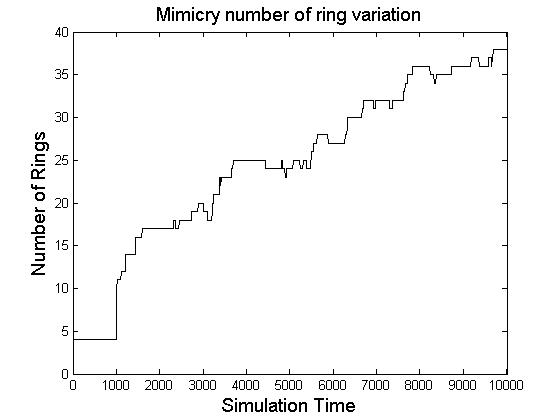
\includegraphics[scale=0.40]{images/ringSize10k-4MorePrey}
	\caption[Number of mimicry rings (4 prey species, increased population)]{Number of mimicry rings, initialized with 4 prey species with increased population.}
	\label{fig:ringSize10k-4MorePrey}
\end{figure}

\section{Initial population with six prey species}
\label{sec:init-conf-6-prey}
\begin{table}[H]
\centering
\begin{tabular}{|l|l|c|c|l|c|}
  \hline
   														&\multicolumn{3}{|c|}{Prey configuration} 																	
   														& \multicolumn{2}{|c|}{Predator configuration} \\ \hline
  \multirow{6}{*}{Population} & Rule110 (Palatable) & \parbox[c]{2.1em}{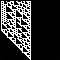
\includegraphics[scale=0.50]{images/CARule110}} 
  																									& 150 & \multicolumn{2}{|c|}{\multirow{6}{*}{30}} \\ \cline{2-4}
  					 									& Rule30  (Unpalatable)& \parbox[c]{2.1em}{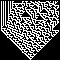
\includegraphics[scale=0.50]{images/CARule30}}  
  					 																				& 150 & \multicolumn{2}{|c|}{}\\ \cline{2-4}
  					 									& Rule55  (Palatable)& \parbox[c]{2.1em}{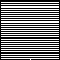
\includegraphics[scale=0.50]{images/CARule55}}    
  					 																				& 150 & \multicolumn{2}{|c|}{}\\ \cline{2-4}
  					 									& Rule190 (Unpalatable)& \parbox[c]{2.1em}{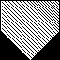
\includegraphics[scale=0.50]{images/CARule190}} 
  					 																				& 150 & \multicolumn{2}{|c|}{}\\ \cline{2-4}
  					 									& Rule57  (Palatable)& \parbox[c]{2.1em}{
\includegraphics[scale=0.50]{images/CARule57}}    
  					 																				& 150 & \multicolumn{2}{|c|}{}\\ \cline{2-4}
  					 									& Rule105 (Unpalatable)& \parbox[c]{2.1em}{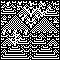
\includegraphics[scale=0.50]{images/CARule105}}& 150 & \multicolumn{2}{|c|}{}\\ \hline
  \multirow{2}{*}{Reproduction} & Age Limit & \multicolumn{2}{|c|}{100}  & \multicolumn{2}{|c|}{500} \\ \cline{2-6}
  						 									& Interval  & \multicolumn{2}{|c|}{1000} & \multicolumn{2}{|c|}{2000} \\ \hline
  \multirow{2}{*}{Mutation Rate} & Pattern   & \multicolumn{2}{|c|}{0.05} & \multicolumn{2}{|c|}{\multirow{2}{*}{0.3}} \\ \cline{2-4}
  						 									 & Genome    & \multicolumn{2}{|c|}{0.5}  & \multicolumn{2}{|c|}{} \\ \hline
  Demise Age	 									 & \multicolumn{3}{|c|}{2000}							& \multicolumn{2}{|c|}{7000} \\ \hline
  Minimum Attack Age						 & \multicolumn{3}{|c|}{} 						    & \multicolumn{2}{|c|}{500} \\ \hline
  \multirow{2}{*}{Memory Configuration} & \multicolumn{3}{|c|}{} 					& Minimum & 6 \\ \cline{5-6}
   																			& \multicolumn{3}{|c|}{} 					& Maximum & 10 \\ \hline  
\end{tabular}
\caption{Agent configuration of 6 prey species.}
\label{tab:config-table-6-prey}
\end{table}

To evaluate the simulation at a more complex level we increase the prey population to 900, consisting of 6 different species with very different pattern configuration. To boost predator-prey interaction we also increase the number of predator population to 30. Predator reproduction interval has been set comparatively lower in this simulation to 2000 iteration similar to the demise age which is set to 5000. As the initial population of prey species is very high, over time we are expecting even larger number of prey species. If predator population does not increase at similar rate there might be a prey population explosion were predator will have no effect on providing selection pressure for the evolution of mimicry. So that is why predator population control parameter has been set to this level. For memory configuration, the minimum number is set to 6, meaning the predator will have to store 6 different prey pattern configuration before starting to make intelligent decision about consuming them. As previously mentioned this number is always set in accordance with the initial number of different prey configuration. 

\begin{figure}[H]
	\centering
	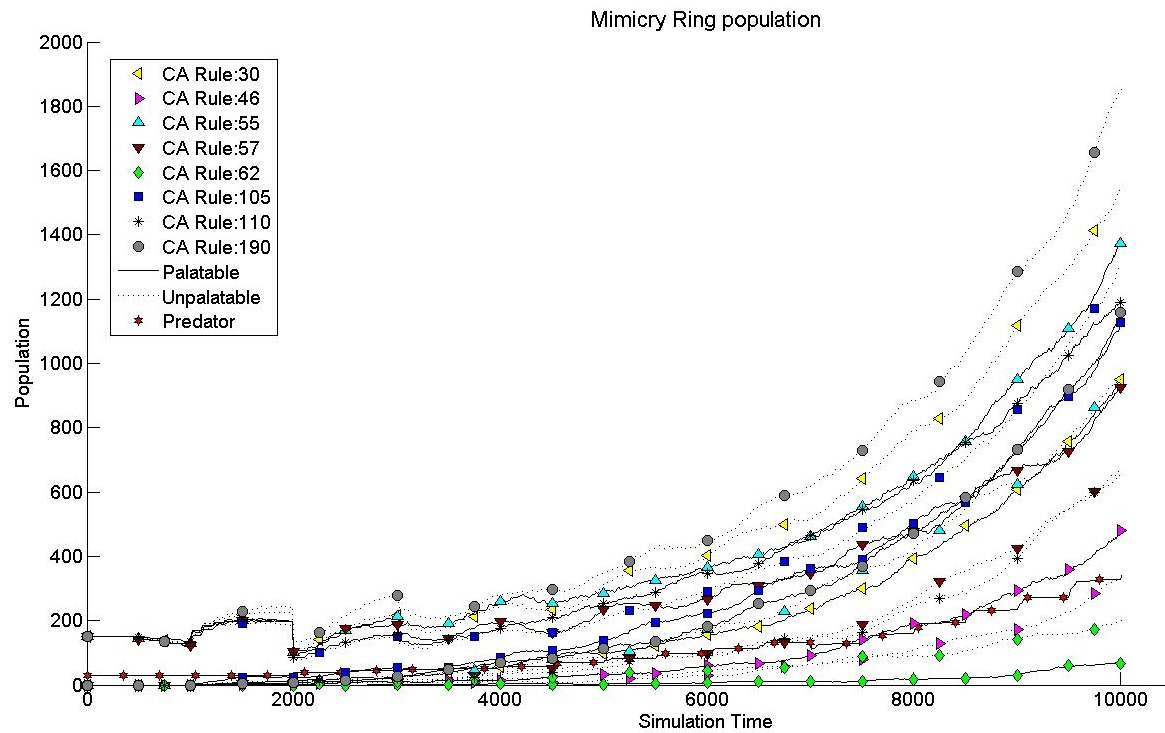
\includegraphics[scale=0.45]{images/simTime10k-6Prey}
	\caption[Population distribution of mimicry rings (6 prey species)]{Population distribution of mimicry rings, initialized with 6 prey species.}
	\label{fig:plot-6-prey}
\end{figure}

With the above set of parameters we receive the plot of figure \ref{fig:plot-6-prey}. An enormous diversity of species can be observed from this experiment. In addition to the six prey species with which the simulation starts, the total number of mimicry rings reach nearly 50. Observing the top 8 as presented in the plot of figure \ref{fig:plot-6-prey}, effects of Batesian mimicry is obvious. Unpalatable CA Rule 190 and 30 dominates the population. Similarly unpalatable CA Rule 105 is also dominant. But after 10000 iterations CA Rule 55 seems to have higher population than 105 even though 55 is a \textsl{palatable} set of species. This anomaly could be the reason for storing large number of patterns in the predator Hopfiled memory. As we know that the number of patterns stored in Hopfiled network is inversely proportional to its recognition rate. In this simulation memory size is controlled by the `Maximum Memory Configuration' which is set to 10 in table \ref{tab:config-table-6-prey}. Also it seems from this experiment that the `Minimum Memory Configuration' being 6 is rather a large number. So there could be possibility of wrong recognition by Hopfield memory. Then again this phenomenon is common if we consider behavior of predators in nature. It is definitely hard for a single predator to memorize multiple poisonous patterns and because of which Mullerian mimicry takes an effect as mentioned in section \ref{sec:mullerian-mimicry}.

\begin{figure}[H]
	\centering
	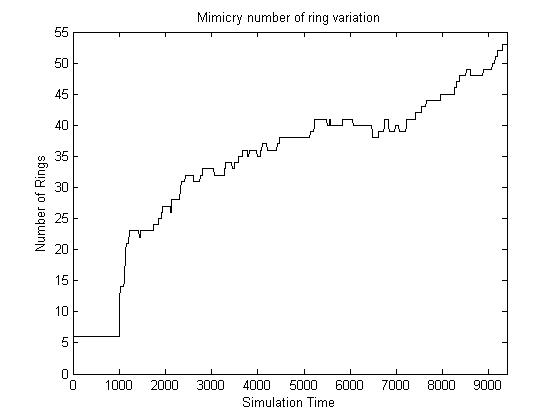
\includegraphics[scale=0.50]{images/ringSize10k-6Prey}
	\caption[Number of mimicry rings (6 prey species)]{Number of mimicry rings, initialized with 6 prey species.}
	\label{fig:ringSize10k-6-Prey}
\end{figure}

\section{Initial configuration with only unpalatable species}
\label{sec:init-conf-only-unp}
\begin{table}[H]
\centering
\begin{tabular}{|l|l|c|c|l|c|}
  \hline
   														&\multicolumn{3}{|c|}{Prey configuration} 																	
   														& \multicolumn{2}{|c|}{Predator configuration} \\ \hline
  \multirow{4}{*}{Population} & Rule110 (Unpalatable) & \parbox[c]{2.1em}{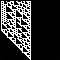
\includegraphics[scale=0.50]{images/CARule110}} 
  																									& 150 & \multicolumn{2}{|c|}{\multirow{4}{*}{20}} \\ \cline{2-4}
  					 									& Rule30  (Unpalatable)& \parbox[c]{2.1em}{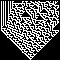
\includegraphics[scale=0.50]{images/CARule30}}  
  					 																				& 150 & \multicolumn{2}{|c|}{}\\ \cline{2-4}
  					 									& Rule55  (Unpalatable)& \parbox[c]{2.1em}{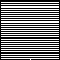
\includegraphics[scale=0.50]{images/CARule55}}    
  					 																				& 150 & \multicolumn{2}{|c|}{}\\ \cline{2-4}
  					 									& Rule190 (Unpalatable)& \parbox[c]{2.1em}{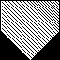
\includegraphics[scale=0.50]{images/CARule190}}& 150 & \multicolumn{2}{|c|}{}\\ \hline
  \multirow{2}{*}{Reproduction} & Age Limit & \multicolumn{2}{|c|}{100}  & \multicolumn{2}{|c|}{500} \\ \cline{2-6}
  						 									& Interval  & \multicolumn{2}{|c|}{1000} & \multicolumn{2}{|c|}{2000} \\ \hline
  \multirow{2}{*}{Mutation Rate} & Pattern   & \multicolumn{2}{|c|}{0.05} & \multicolumn{2}{|c|}{\multirow{2}{*}{0.3}} \\ \cline{2-4}
  						 									 & Genome    & \multicolumn{2}{|c|}{0.5}  & \multicolumn{2}{|c|}{} \\ \hline
  Demise Age	 									 & \multicolumn{3}{|c|}{2000}							& \multicolumn{2}{|c|}{5000} \\ \hline
  Minimum Attack Age						 & \multicolumn{3}{|c|}{} 						    & \multicolumn{2}{|c|}{500} \\ \hline
  \multirow{2}{*}{Memory Configuration} & \multicolumn{3}{|c|}{} 					& Minimum & 4 \\ \cline{5-6}
   																			& \multicolumn{3}{|c|}{} 					& Maximum & 10 \\ \hline  
\end{tabular}
\caption{Agent configuration of 4 prey species all unpalatable.}
\label{tab:config-table-4-prey-unpalatable}
\end{table}

To further observe the effects of mimicry ring we initialize the simulation with all unpalatable prey species. After finding different anomalous behavior of predator recognition capability in section \ref{sec:init-conf-6-prey} for increased number of diverse prey species; for this experiment the initial number of species have been reduced from six to four. As explained earlier the minimum memory configuration is also set to four in accordance to the initial number of prey species. Rest of the parameters remain quite unchanged.

\begin{figure}[H]
	\centering
	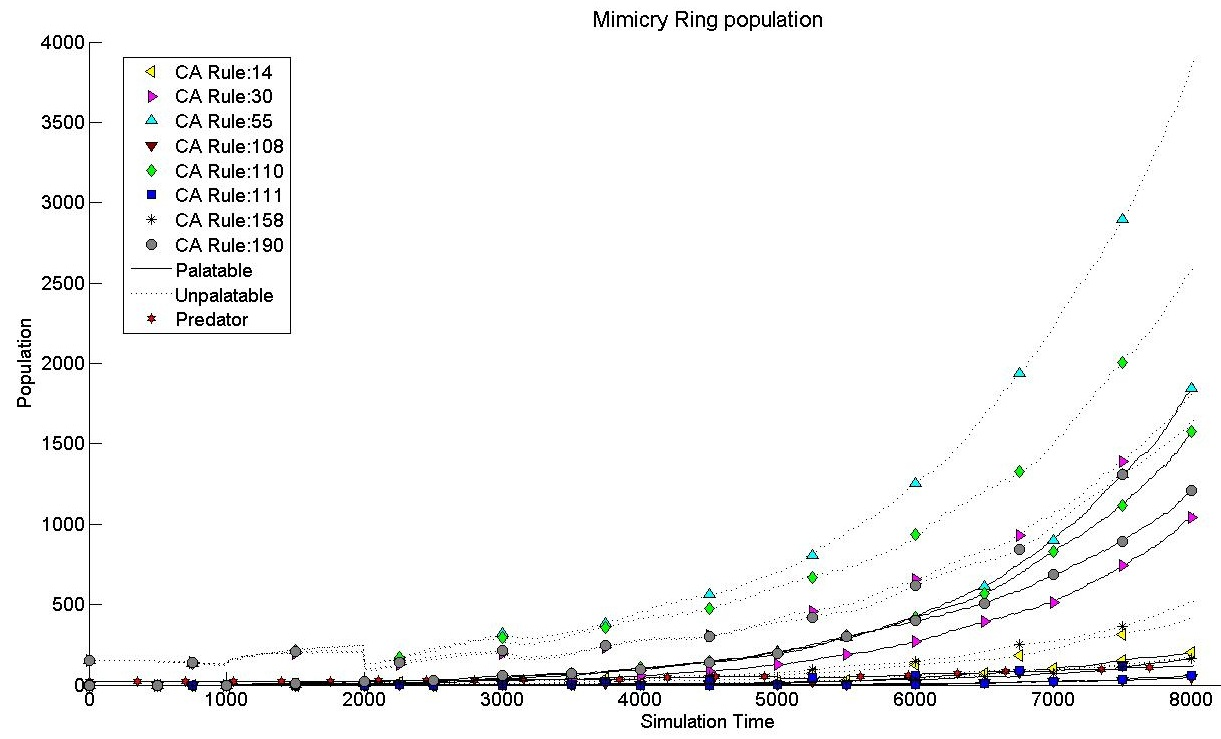
\includegraphics[scale=0.45]{images/simTime8k-4Prey-unp}
	\caption[Population distribution of mimicry rings(4 prey species all unpalatable)]{Population distribution of mimicry rings, initialized with 4 prey species all unpalatable.}
	\label{fig:plot-4-prey-unp}
\end{figure}

The results according to figure \ref{fig:plot-4-prey-unp} are much expected. The population of unpalatable species have prevailed. After nearly 8000 iterations we can see unpalatable species of CA rule 55, 110, 30 and 190 have prevailed with the most population. All of their palatable counter parts are also increasing their population deceiving the predators. We observe the effect of the simulation up to 8000 iterations instead of 10000 as the total number of prey species increases at an enormous rate in this simulation within very short period of time. As most of the species are unpalatable, predators mostly do not get the opportunity to consume, causing a much lower prey death rate. 

\begin{figure}[H]
	\centering
	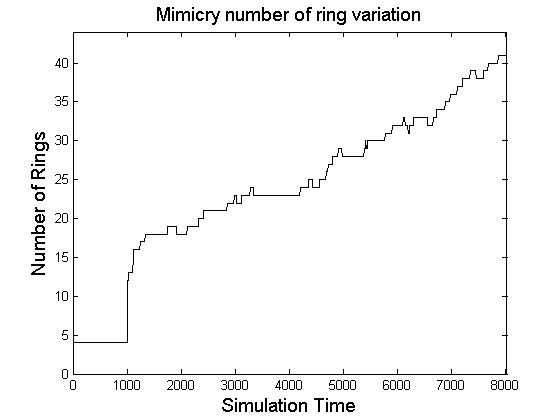
\includegraphics[scale=0.50]{images/ringSize8k-4Prey-unp}
	\caption[Number of mimicry rings (4 prey species all unpalatable)]{Number of mimicry rings, initialized with 4 prey species all unpalatable.}
	\label{fig:ringSize10k-4-Prey-unp}
\end{figure}

This experiment is an ideal scenario for observing Mullerian mimicry. As mentioned in section \ref{sec:mullerian-mimicry}, Mullerian mimicry occurs between multiple species of unpalatable prey population. From the second work of Franks and Noble \cite{franks2003} mentioned in section \ref{subsec:models-by-frank-and-noble}, we note that multiple Mullerian mimicry rings are expected to converge into one large ring through the evolutionary process of punctuated equilibrium. But in this experiment as the predator's `Minimum Memory Configuration' is set to four, all predators have the capability to recognize four prey patterns before starting to make intelligent decision of consuming them. By setting `Minimum Memory Configuration' to one, also increasing `Predator Demise Age' to 7000 and decreasing predator's `Reproduction Age Interval' to 1500, we get the following plot. 

\begin{figure}[H]
	\centering
	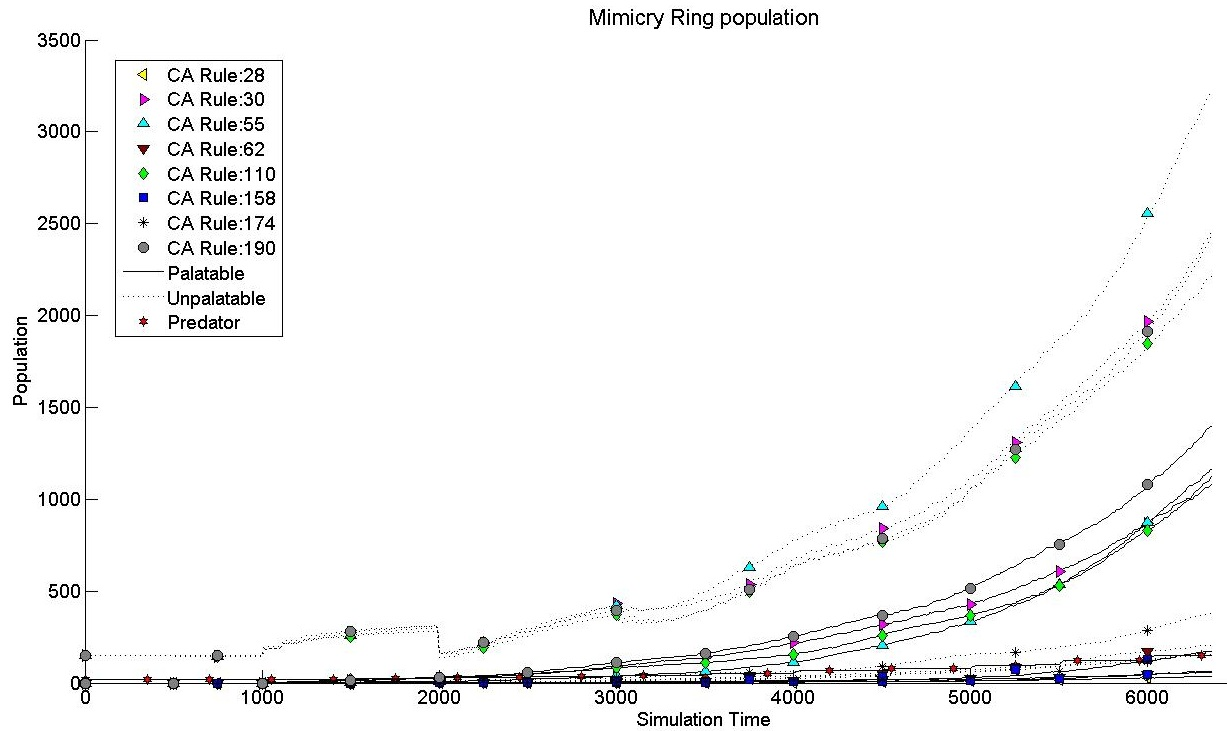
\includegraphics[scale=0.45]{images/simTime6k-4Prey-unp-1-mem}
	\caption[Population distribution of mimicry rings(4 prey, all unpalatable but reduced predator memory)]{Population distribution of mimicry rings, initialized with 4 prey species all unpalatable. Minimum Memory size reduced to one.}
	\label{fig:plot-4-prey-unp-1-mem}
\end{figure}

Running the simulation for 6000 iterations there was no sign for all prey population to converge into one large ring. As it can be observed in figure \ref{fig:plot-4-prey-unp-1-mem} all four unpalatable prey population have a very dominant presence in the simulation. Even though predator minimum memory has been reduced to only one pattern, different population of predators become familiar with different prey patterns, which results in the existence of multiple Mullerian mimicry ring instead of a single one.

\section{Initial configuration with only palatable species}
\label{sec:init-only-palatable-species}

\begin{table}[H]
\centering
\begin{tabular}{|l|l|c|c|l|c|}
  \hline
   														&\multicolumn{3}{|c|}{Prey configuration} 																	
   														& \multicolumn{2}{|c|}{Predator configuration} \\ \hline
  \multirow{4}{*}{Population} & Rule110 (Palatable) & \parbox[c]{2.1em}{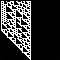
\includegraphics[scale=0.50]{images/CARule110}} 
  																									& 150 & \multicolumn{2}{|c|}{\multirow{4}{*}{20}} \\ \cline{2-4}
  					 									& Rule30  (Palatable)& \parbox[c]{2.1em}{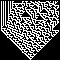
\includegraphics[scale=0.50]{images/CARule30}}  
  					 																				& 150 & \multicolumn{2}{|c|}{}\\ \cline{2-4}
  					 									& Rule55  (Palatable)& \parbox[c]{2.1em}{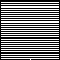
\includegraphics[scale=0.50]{images/CARule55}}    
  					 																				& 150 & \multicolumn{2}{|c|}{}\\ \cline{2-4}
  					 									& Rule190 (Palatable)& \parbox[c]{2.1em}{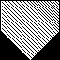
\includegraphics[scale=0.50]{images/CARule190}}& 150 & \multicolumn{2}{|c|}{}\\ \hline
  \multirow{2}{*}{Reproduction} & Age Limit & \multicolumn{2}{|c|}{100}  & \multicolumn{2}{|c|}{500} \\ \cline{2-6}
  						 									& Interval  & \multicolumn{2}{|c|}{1000} & \multicolumn{2}{|c|}{2000} \\ \hline
  \multirow{2}{*}{Mutation Rate} & Pattern   & \multicolumn{2}{|c|}{0.05} & \multicolumn{2}{|c|}{\multirow{2}{*}{0.3}} \\ \cline{2-4}
  						 									 & Genome    & \multicolumn{2}{|c|}{0.5}  & \multicolumn{2}{|c|}{} \\ \hline
  Demise Age	 									 & \multicolumn{3}{|c|}{2000}							& \multicolumn{2}{|c|}{5000} \\ \hline
  Minimum Attack Age						 & \multicolumn{3}{|c|}{} 						    & \multicolumn{2}{|c|}{500} \\ \hline
  \multirow{2}{*}{Memory Configuration} & \multicolumn{3}{|c|}{} 					& Minimum & 4 \\ \cline{5-6}
   																			& \multicolumn{3}{|c|}{} 					& Maximum & 10 \\ \hline  
\end{tabular}
\caption{Agent configuration of 4 prey species all palatable.}
\label{tab:config-table-4-prey-palatable}
\end{table}

The parameters for this simulation has been set exactly the same as in table \ref{tab:config-table-4-prey-unpalatable} except all the species are palatable at this point. All predator configuration has also been set to exactly same as before.

The results for the configuration in table \ref{tab:config-table-4-prey-palatable} can be observed in figure \ref{fig:plot-4-prey-p} where all population of prey species have reached its demise at nearly 7000 iterations. By analyzing details we can see, around simulation time 500 all population of species come to a steady downfall as at this point initial predator species reach its' age for consumption. Around simulation time 1000 all population of prey species start increasing steadily because they reach their maturity level of reproduction. At iteration time 2000 there is a sudden drop of prey population because the initial population of prey have reached its demise age at this point. By this time the population of unpalatable species mutated from the palatable ones start increasing, and slowly around time 7000 and onwards the entire population of prey come to its demise. Predator population, from the beginning of the simulation has taken a very dominant effect. As all the species are palatable, predator's consumption and reproduction rate is extremely high and it keep increasing in a geometric rate.

\begin{figure}[H]
	\centering
	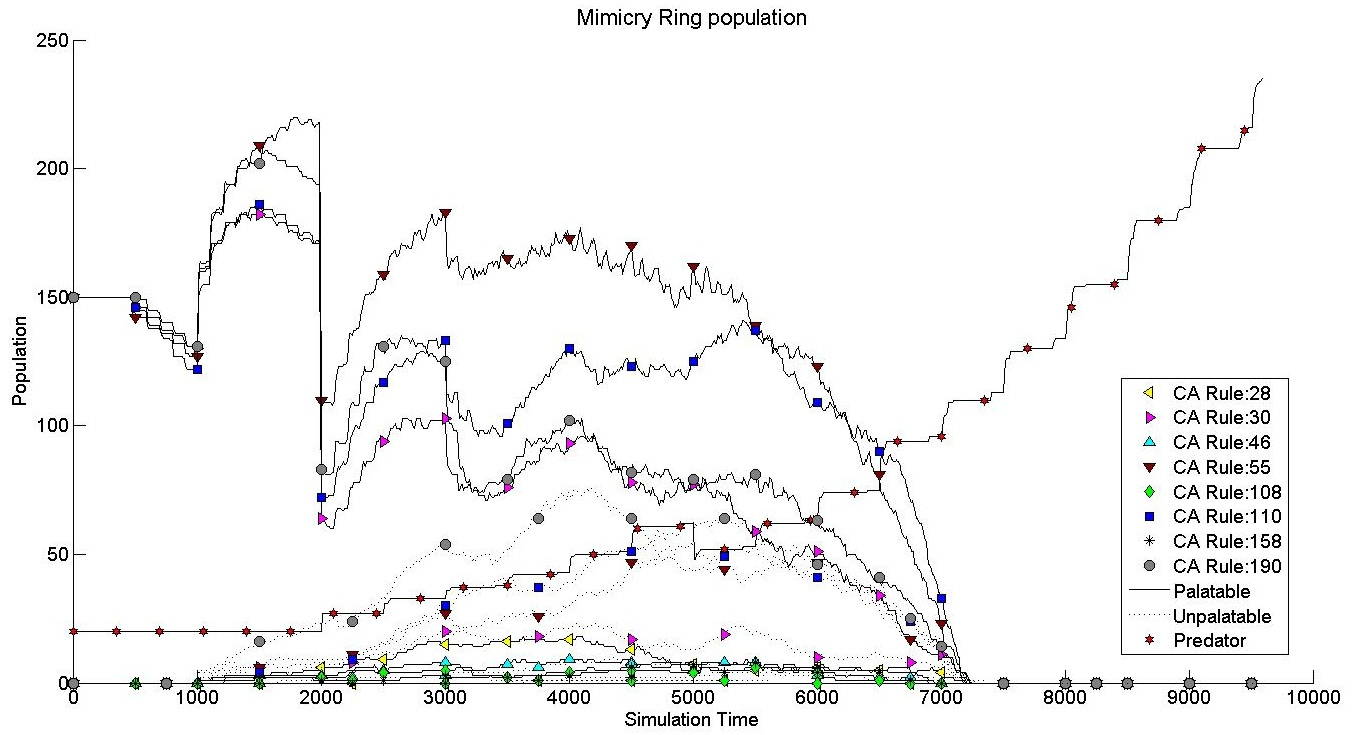
\includegraphics[scale=0.40]{images/simTime10k-4Prey-p}
	\caption[Population distribution of mimicry rings (4 prey species all palatable)]{Population distribution of mimicry rings, initialized with 4 prey species all palatable.}
	\label{fig:plot-4-prey-p}
\end{figure}

\begin{figure}[H]
	\centering
	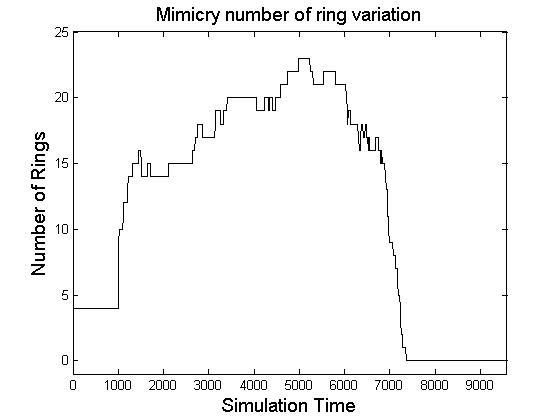
\includegraphics[scale=0.50]{images/ringSize10k-4Prey-p}
	\caption[Number of mimicry rings (4 prey species all palatable)]{Number of mimicry rings, initialized with 4 prey species all palatable.}
	\label{fig:ringSize8k-4-Prey-p}
\end{figure}

Observation of mimicry rings also tell us about the results we have seen in the plot of figure \ref{fig:plot-4-prey-p}. The number of rings keep increasing but comes to a sudden drop around simulation time 7000 and goes to zero.

\section{Initial configuration with single prey species}
Until now all experiments have been initialized with multiple prey species. The following set of experiments have been initialized with only a single prey species, for both cases of unpalatable and palatable.

\subsection{Unpalatable}
\label{subsec:single-prey-unpalatable}

\begin{table}[H]
\centering
\begin{tabular}{|l|l|c|c|l|c|}
  \hline
   														&\multicolumn{3}{|c|}{Prey configuration} 																	
   														& \multicolumn{2}{|c|}{Predator configuration} \\ \hline
  Population 									& Rule30 (Unpalatable) & \parbox[c]{2.1em}{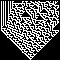
\includegraphics[scale=0.50]{images/CARule30}} 
  																									& 216 & \multicolumn{2}{|c|}{10} \\ \hline
  \multirow{2}{*}{Reproduction} & Age Limit & \multicolumn{2}{|c|}{100}  & \multicolumn{2}{|c|}{500} \\ \cline{2-6}
  						 									& Interval  & \multicolumn{2}{|c|}{1000} & \multicolumn{2}{|c|}{2500} \\ \hline
  \multirow{2}{*}{Mutation Rate} & Pattern   & \multicolumn{2}{|c|}{0.05} & \multicolumn{2}{|c|}{\multirow{2}{*}{0.3}} \\ \cline{2-4}
  						 									 & Genome    & \multicolumn{2}{|c|}{0.5}  & \multicolumn{2}{|c|}{} \\ \hline
  Demise Age	 									 & \multicolumn{3}{|c|}{2000}							& \multicolumn{2}{|c|}{7000} \\ \hline
  Minimum Attack Age						 & \multicolumn{3}{|c|}{} 						    & \multicolumn{2}{|c|}{500} \\ \hline
  \multirow{2}{*}{Memory Configuration} & \multicolumn{3}{|c|}{} 					& Minimum & 2 \\ \cline{5-6}
   																			& \multicolumn{3}{|c|}{} 					& Maximum & 10 \\ \hline  
\end{tabular}
\caption{Agent configuration of 1 prey species unpalatable.}
\label{tab:config-table-1-prey-unpalatable}
\end{table}

This configuration has only one unpalatable species, one in each of the 216 cells, equally distributed all over the environment. Also have a set of 10 predators. Their minimum memory configuration has been set to 2 as any value below 2 will not help the Hopfield Network Memory to differentiate between two patterns.

\begin{figure}[H]
	\centering
	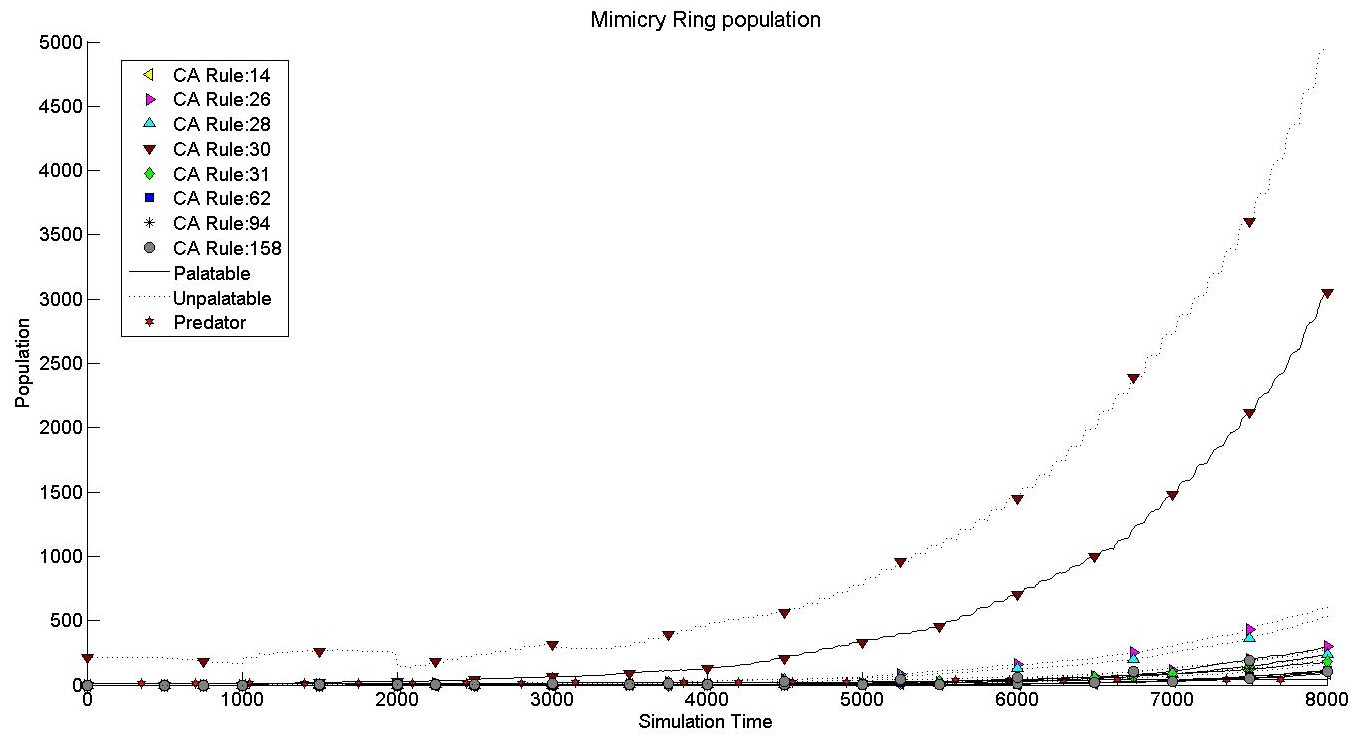
\includegraphics[scale=0.40]{images/simTime8k-1Prey-unp}
	\caption[Population distribution of mimicry rings (1 prey species unpalatable)]{Population distribution of mimicry rings, initialized with 1 prey species unpalatable.}
	\label{fig:plot-1-prey-unp}
\end{figure}

From figure \ref{fig:plot-1-prey-unp}, it can be observed, the initial set of unpalatable species is dominant as expected. The palatable population mimicking that set is following it. A bunch of other rings with majority of unpalatable species have been reproduced through mutation. Mainly because the initial population started with a bunch of unpalatable species, so their reproduced generation have similar behavior as well.

\begin{figure}[H]
	\centering
	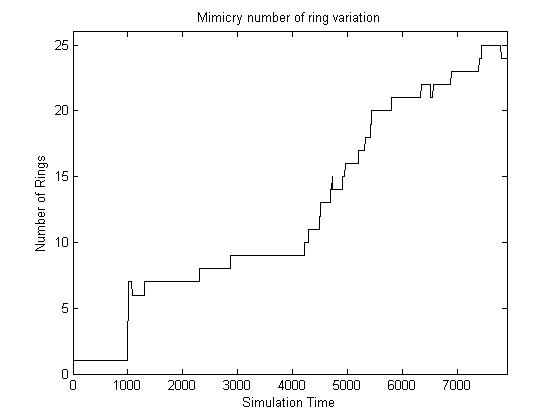
\includegraphics[scale=0.50]{images/ringSize8k-1Prey-unp}
	\caption[Number of mimicry rings (1 prey species unpalatable)]{Number of mimicry rings, initialized with 1 prey species unpalatable.}
	\label{fig:ringSize8k-1-Prey-unp}
\end{figure}

\subsection{Palatable}
\begin{table}[H]
\centering
\begin{tabular}{|l|l|c|c|l|c|}
  \hline
   														&\multicolumn{3}{|c|}{Prey configuration} 																	
   														& \multicolumn{2}{|c|}{Predator configuration} \\ \hline
  Population 									& Rule30 (Palatable) & \parbox[c]{2.1em}{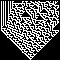
\includegraphics[scale=0.50]{images/CARule30}} 
  																									& 216 & \multicolumn{2}{|c|}{8} \\ \hline
  \multirow{2}{*}{Reproduction} & Age Limit & \multicolumn{2}{|c|}{100}  & \multicolumn{2}{|c|}{500} \\ \cline{2-6}
  						 									& Interval  & \multicolumn{2}{|c|}{1000} & \multicolumn{2}{|c|}{2500} \\ \hline
  \multirow{2}{*}{Mutation Rate} & Pattern   & \multicolumn{2}{|c|}{0.05} & \multicolumn{2}{|c|}{\multirow{2}{*}{0.3}} \\ \cline{2-4}
  						 									 & Genome    & \multicolumn{2}{|c|}{0.5}  & \multicolumn{2}{|c|}{} \\ \hline
  Demise Age	 									 & \multicolumn{3}{|c|}{2000}							& \multicolumn{2}{|c|}{7000} \\ \hline
  Minimum Attack Age						 & \multicolumn{3}{|c|}{} 						    & \multicolumn{2}{|c|}{500} \\ \hline
  \multirow{2}{*}{Memory Configuration} & \multicolumn{3}{|c|}{} 					& Minimum & 2 \\ \cline{5-6}
   																			& \multicolumn{3}{|c|}{} 					& Maximum & 10 \\ \hline  
\end{tabular}
\caption{Agent configuration of 1 prey species palatable.}
\label{tab:config-table-1-prey-palatable}
\end{table}

This configuration is set exactly as according to section \ref{subsec:single-prey-unpalatable} but with a single set of palatable species. The population of predators have been reduced from 10 to 8 to avoid elimination of all prey species as it happened in case of section \ref{sec:init-only-palatable-species}.

\begin{figure}[H]
	\centering
	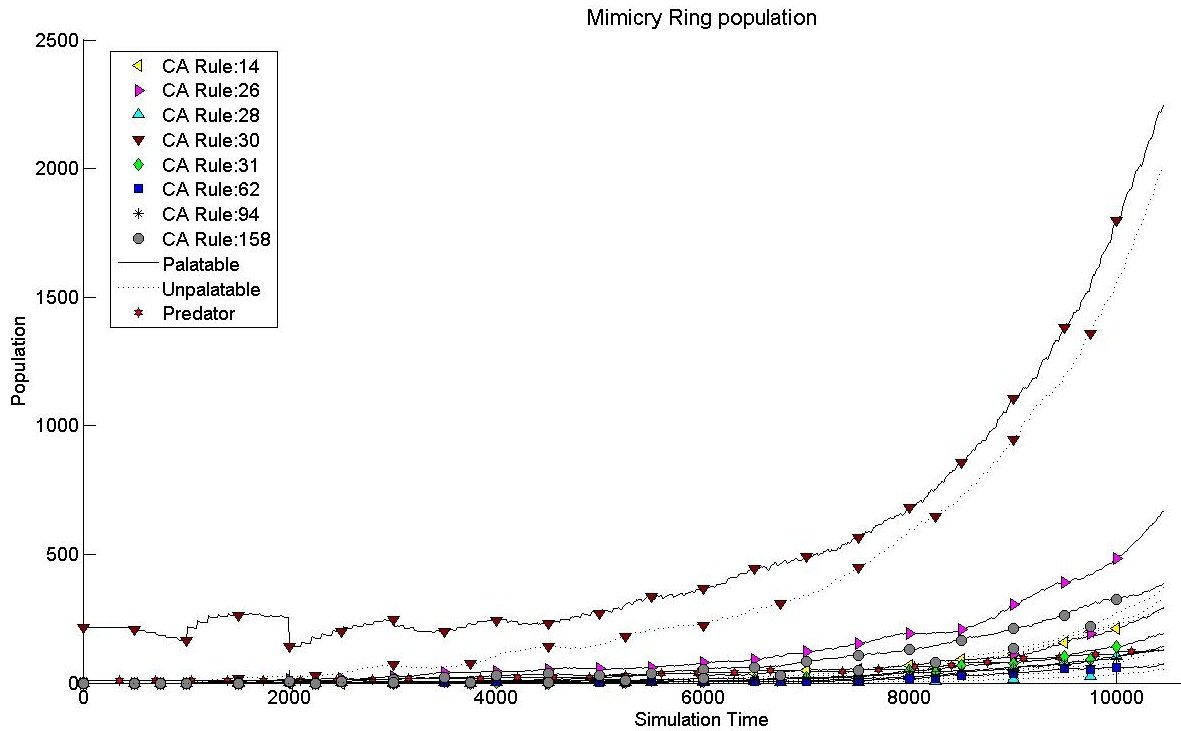
\includegraphics[scale=0.45]{images/simTime10k-1Prey-p}
	\caption[Population distribution of mimicry rings (1 prey species palatable)]{Population distribution of mimicry rings, initialized with 1 prey species palatable.}
	\label{fig:plot-1-prey-p}
\end{figure}

From the initial palatable population we see a bunch of palatable rings created. Major difference from section \ref{subsec:single-prey-unpalatable} is the total number of prey population created. For the unpalatable species in section \ref{subsec:single-prey-unpalatable}, total prey population reach above 12 thousand. But for palatable species total population reach nearly above 5000 prey species, as when the preys are palatable there is more consumption from predators. 

\begin{figure}[H]
	\centering
	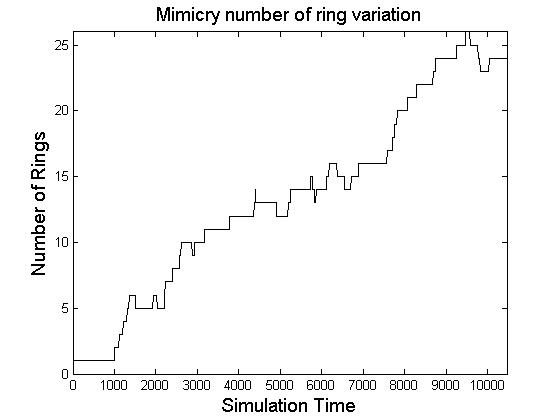
\includegraphics[scale=0.50]{images/ringSize10k-1Prey-p}
	\caption[Number of mimicry rings (1 palatable prey species)]{Number of mimicry rings, initialized with 1 palatable prey species.}
	\label{fig:ringSize8k-1-Prey-p}
\end{figure}

\section{Analysis of Batesian Mimicry}
\label{sec:result-batesian-mimicry}
For all possible initial conditions, Batesian mimicry has taken effect. It can be observed that for every ring of unpalatable species there is an existence of the palatable ring racing to reach the population count of its unpalatable counterpart. Also when the initial population starts with a set of only palatable species we can observe that the total population vanishes within very short period of time (section \ref{sec:init-only-palatable-species}). This effect can be explained with the fact that the palatable population does not have any models to mimic, and it reaches extinction. So from this analysis it can be concluded that the model under discussion has successfully simulated the evolution of Batesian mimicry.

\section{Analysis of Mullerian Mimicry}
\label{sec:result-mullerian-mimicry}
Effects of Mullerian mimicry can be observed best for the experiment in section \ref{sec:init-conf-only-unp}. For that case, we initialized the model with 4 rings of unpalatable species with no palatable ones and after nearly 10K iterations, all of the initial unpalatable rings have survived with dominance. The cause of this behavior can be explained by the minimum number of patterns that each predator can store in memory, which was set to four. So this parameter was reduced to one to observe whether it is possible to converge all different unpalatable rings into one large ring, when predators are capable to memorizing only a single pattern. But as it turned out, the phenomena of ``a single large ring" does not occur because different predators recognize different patterns resulting in multiple divergent Mullerian mimicry rings. It can be concluded that our results match with the one from Franks and Noble (section \ref{subsec:models-by-frank-and-noble}), that multiple Mullerian mimics do not converge into one large ring.

\section{Conclusion}
\label{sec:result-conclusion}
Analysis of the results tell us that we have successfully been able to simulate the evolution of mimicry. In addition to that, this model provides a more accurate simulation of the fascinating natural process of mimicry rings. Not only does this model simulates mimicry with the initialized population but also it provides possibility of creating diverse new rings and their shift in population. This model also proves the theory of Turner in explaining the evolution of mimicry with punctuated equilibrium (section \ref{subsec:reflection-of-punctuated-equilibrium}) \cite{turner1988}.